% 1D Dirichlet sine decay -- case_1d.py (thermal_scalar, pure operator).
% Domain [0,L], both walls held isothermal at Twall; initial half-sine bump
% T_s(x,0) = Twall + A sin(pi x/L) decays in place toward Twall with no flow.
%
% Compile:  pdflatex setup_1d_dirichlet.tex
\documentclass[border=6pt]{standalone}
\usepackage{amsmath}
\usepackage{tikz}
\usepackage{pgfplots}
\pgfplotsset{compat=1.18}
\usetikzlibrary{arrows.meta}

\definecolor{coldc}{RGB}{46,86,149}
\definecolor{hotc}{RGB}{171,57,52}
\definecolor{inkc}{RGB}{30,30,30}

\begin{document}
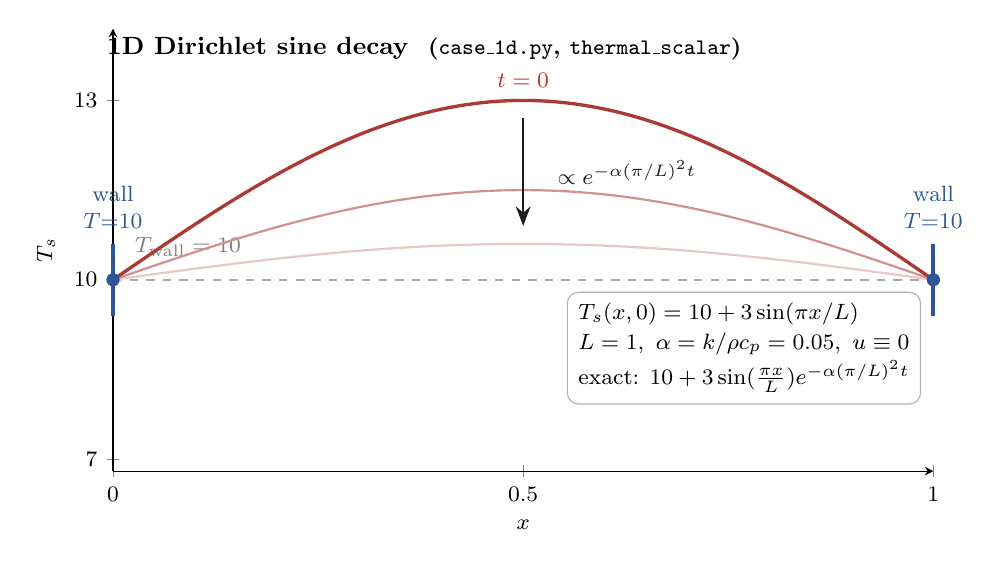
\begin{tikzpicture}[>=Stealth, font=\footnotesize]
\begin{axis}[
  width=12cm, height=7.2cm,
  xlabel={$x$}, ylabel={$T_s$},
  xmin=0, xmax=1, ymin=6.8, ymax=14.2,
  axis lines=left, samples=160,
  xtick={0,0.5,1}, ytick={7,10,13},
  enlargelimits=false, clip=false,
]
  % baseline wall temperature
  \addplot[gray!70, dashed, thick, domain=0:1] {10};
  \node[gray, anchor=west] at (axis cs:0.015,10.55) {$T_{\text{wall}}=10$};

  % decayed profiles (later times, lighter) -> shows in-place decay
  \addplot[hotc!28, thick, domain=0:1] {10 + 3*0.20*sin(deg(pi*x))};
  \addplot[hotc!55, thick, domain=0:1] {10 + 3*0.50*sin(deg(pi*x))};

  % initial profile t = 0
  \addplot[hotc, very thick, domain=0:1] {10 + 3*sin(deg(pi*x))};
  \node[hotc, anchor=south] at (axis cs:0.5,13.05) {$t=0$};

  % decay direction
  \draw[->, inkc, line width=0.9pt] (axis cs:0.5,12.7) -- (axis cs:0.5,10.9);
  \node[inkc, anchor=west] at (axis cs:0.53,11.8) {$\propto e^{-\alpha(\pi/L)^2 t}$};

  % Dirichlet walls: clamped endpoints on the baseline
  \fill[coldc] (axis cs:0,10) circle (2.4pt);
  \fill[coldc] (axis cs:1,10) circle (2.4pt);
  \draw[coldc, line width=1.4pt] (axis cs:0,9.4)--(axis cs:0,10.6);
  \draw[coldc, line width=1.4pt] (axis cs:1,9.4)--(axis cs:1,10.6);
  \node[coldc, anchor=south, align=center] at (axis cs:0,10.7) {wall\\$T{=}10$};
  \node[coldc, anchor=south, align=center] at (axis cs:1,10.7) {wall\\$T{=}10$};

  % parameter box
  \node[draw=inkc!35, rounded corners, align=left, anchor=north east,
        fill=white, inner sep=4pt]
    at (axis cs:0.985,9.8)
    {$T_s(x,0)=10+3\sin(\pi x/L)$\\[1pt]
     $L=1,\ \alpha=k/\rho c_p=0.05,\ u\equiv 0$\\[1pt]
     exact: $10+3\sin(\tfrac{\pi x}{L})e^{-\alpha(\pi/L)^2 t}$};
\end{axis}
\node[font=\bfseries\small, anchor=south west] at (-0.2,5.1)
  {1D Dirichlet sine decay \ \footnotesize(\texttt{case\_1d.py}, \texttt{thermal\_scalar})};
\end{tikzpicture}
\end{document}
